\documentclass[12pt]{article}

\usepackage[a5paper, landscape, margin=10mm]{geometry}
\usepackage{enumitem}
\usepackage{amsmath}
\usepackage{amssymb}
\usepackage{amsfonts}
\usepackage{placeins}
\usepackage{graphicx}
\usepackage{listings}
\usepackage{caption}
\usepackage{colortbl}
\usepackage[parfill]{parskip}
\usepackage[mathscr]{euscript}
\usepackage[usenames,dvipsnames,svgnames,table,hyperref]{xcolor}
\usepackage[hidelinks]{hyperref}
\usepackage{fontspec}
\usepackage{mdframed}

\setsansfont{FreeSans}
\setmonofont{Ubuntu Mono}
\renewcommand{\familydefault}{\sfdefault}

\hyphenation{WebGL}

\definecolor{webColor}{RGB}{0, 108, 174}
\newcommand{\web}[1]{{\color{webColor} \small \url{#1}}}
\newcommand{\webText}[2]{{\color{webColor} \href{#2}{#1}}}
\newcommand{\email}[2]{{\small \color{webColor} \textsf{\href{mailto:#1@#2}{#1[at]#2}}}}
\definecolor{titleColor}{RGB}{179, 0, 149}
\newcommand{\myTitle}[1]{{\large \color{titleColor} \hspace{-4mm} \textbf{\textsf{#1}}}}
\definecolor{subColor}{RGB}{179, 0, 149}
\newcommand{\mySub}[1]{\textsf{\color{subColor}#1}}
\definecolor{keyColor}{RGB}{170, 149, 0}
\newcommand{\myKey}[1]{\textbf{\color{keyColor}#1}}

\definecolor{redBoxFg}{RGB}{255, 0, 0}
\definecolor{redBoxBg}{RGB}{255, 218, 232}
\newcommand{\redBox}[1]{{\color{redBoxFg}\colorbox{redBoxBg}{#1}}}
\definecolor{yellowBoxFg}{RGB}{0, 0, 0}
\definecolor{yellowBoxBg}{RGB}{255, 232, 0}
\newcommand{\yellowBox}[1]{{\color{yellowBoxFg}\colorbox{yellowBoxBg}{#1}}}
\definecolor{greenBoxFg}{RGB}{0, 0, 0}
\definecolor{greenBoxBg}{RGB}{134, 210, 153}
\newcommand{\greenBox}[1]{{\color{greenBoxFg}\colorbox{greenBoxBg}{#1}}}
\definecolor{blueBoxFg}{RGB}{0, 0, 255}
\definecolor{blueBoxBg}{RGB}{218, 232, 255}
\newcommand{\blueBox}[1]{{\color{blueBoxFg}\colorbox{blueBoxBg}{#1}}}
\definecolor{violetBoxFg}{RGB}{0, 0, 0}
\definecolor{violetBoxBg}{RGB}{218, 204, 255}
\newcommand{\violetBox}[1]{{\color{violetBoxFg}\colorbox{violetBoxBg}{#1}}}

\mdfdefinestyle{MyFrame}{%
    linecolor=black,
    outerlinewidth=0pt,
    linewidth=0pt,
    innertopmargin=2.7pt,
    innerbottommargin=0pt,
    innerrightmargin=0pt,
    innerleftmargin=0pt,
        leftmargin = 0pt,
        rightmargin = 0pt}

\definecolor{lightttColor}{RGB}{69, 69, 80}
\newcommand{\lighttt}[1]{{\color{lightttColor}\texttt{#1}}}

\renewcommand*\labelenumi{(\theenumi)}
\renewcommand*{\theenumii}{\roman{enumii}}
\renewcommand*\labelenumii{\theenumii.}

\newcommand{\fixminipage}{\raggedright \setlength{\parskip}{0.3\baselineskip}}
\newcommand{\codeminipage}{\raggedright \setlength{\parskip}{0\baselineskip}}
\sloppy
\pagenumbering{gobble}


\begin{document}

{\hfill \LARGE \textbf{\textsf{Project Spork: EXO GPU}}}

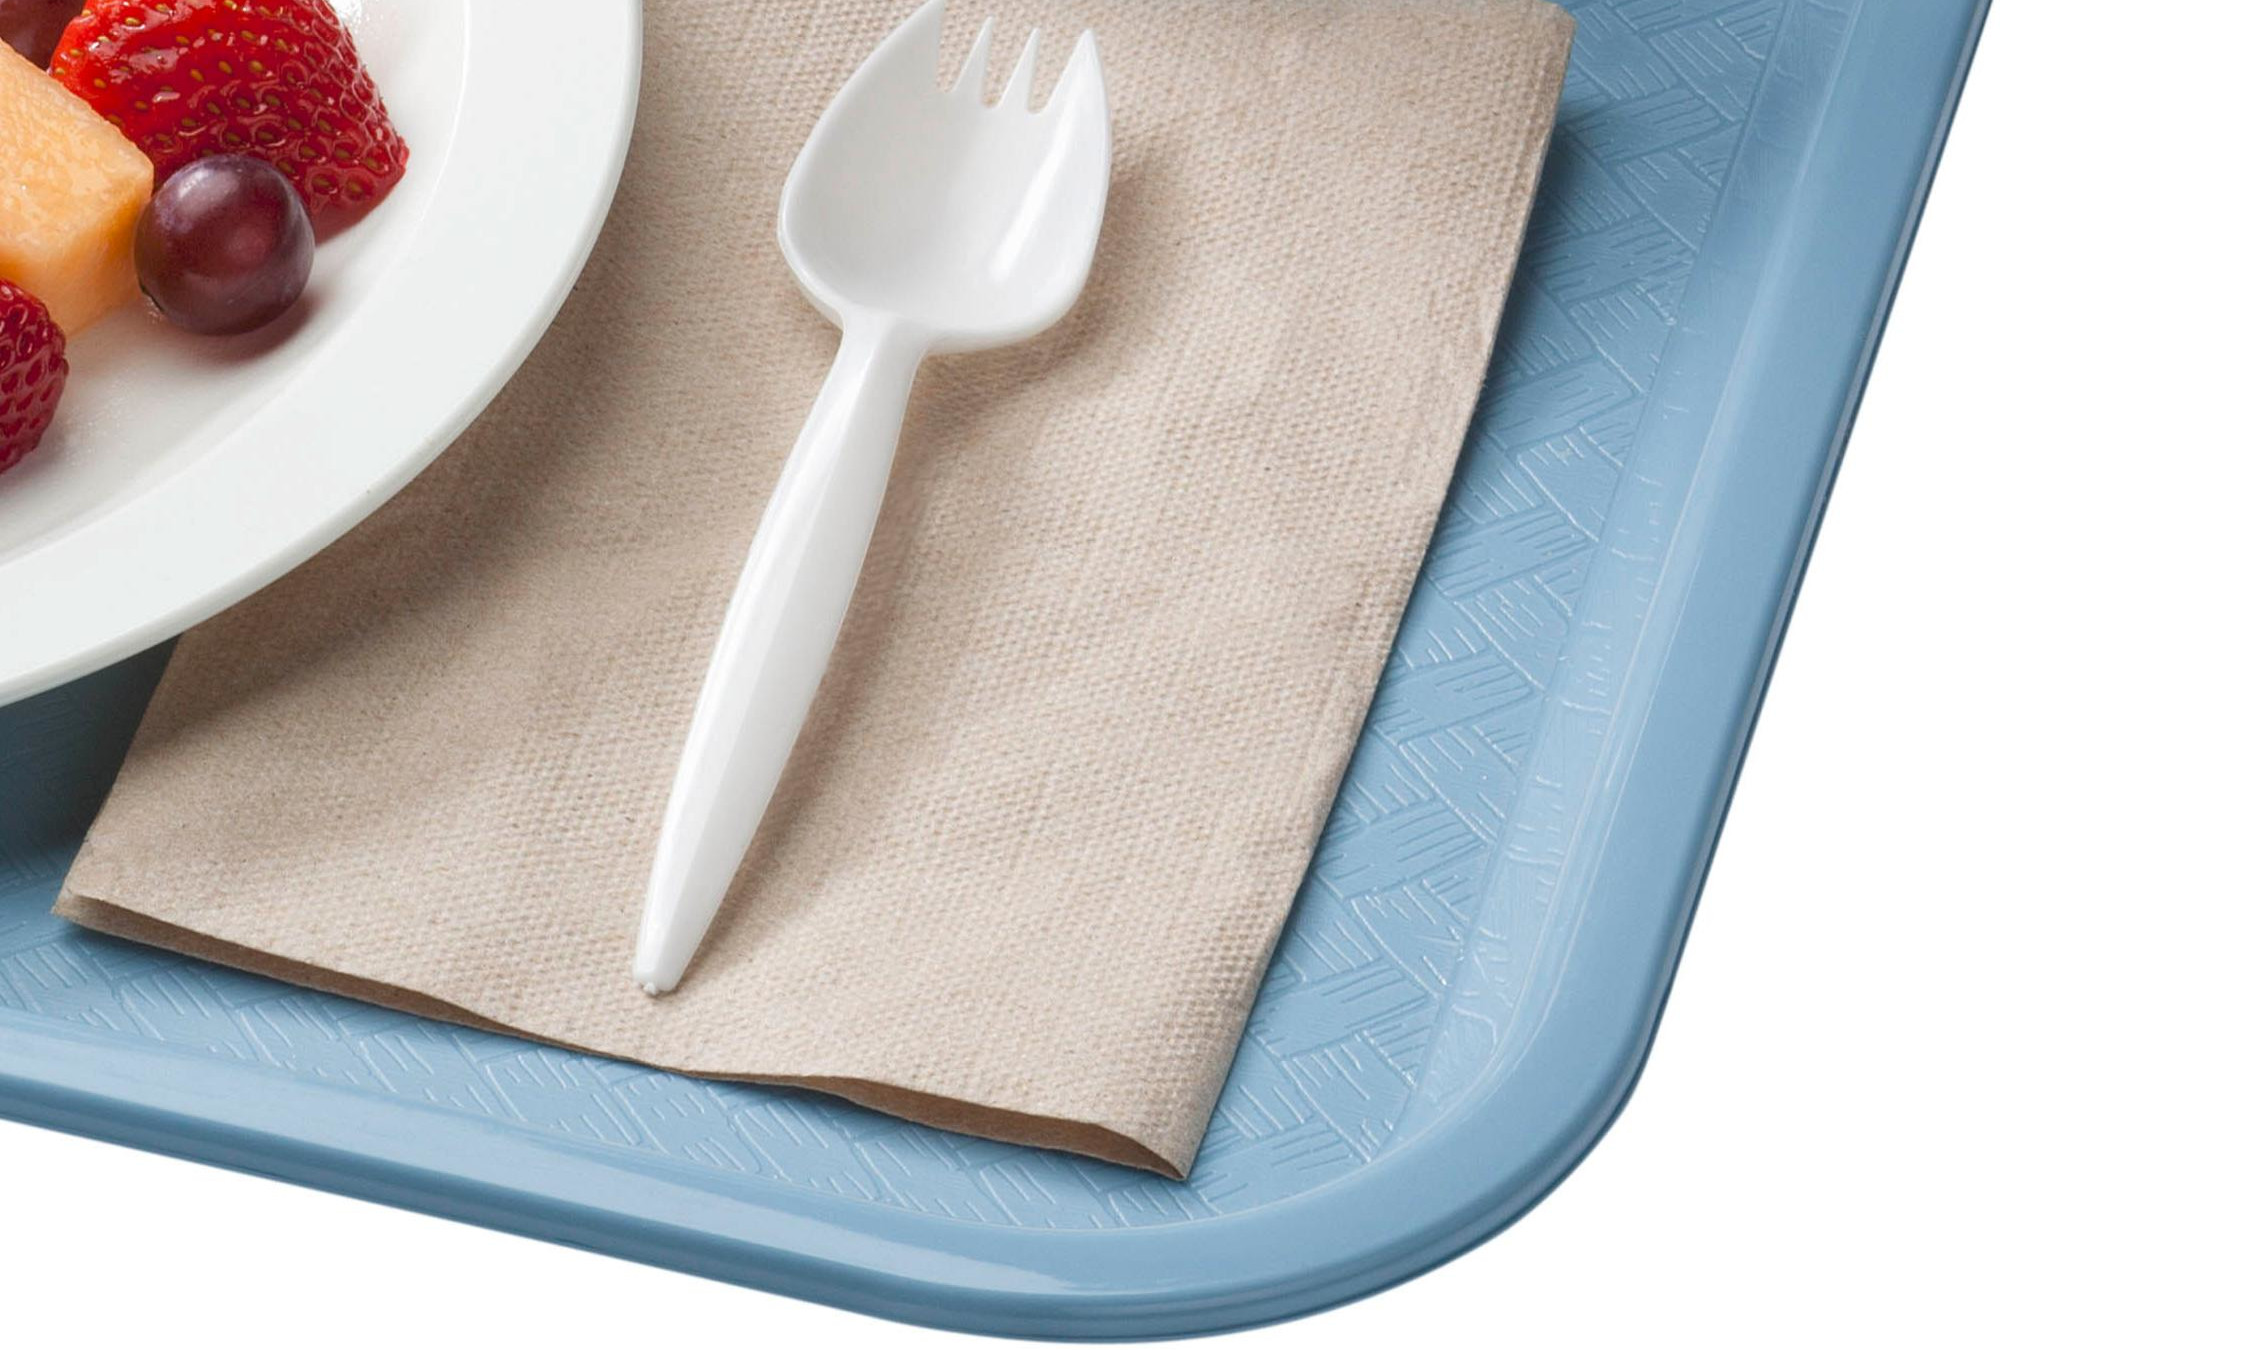
\includegraphics[width=\linewidth]{usda_spork.jpg}

\newpage

\myTitle{Project Goals}

\begin{minipage}[t]{0.5\textwidth}\fixminipage
\myKey{Exo Today:} Python-embedded USL with ``imperative'' rewrite-based scheduling

\texttt{@proc} decorator captures annotated Python AST; procs translated (almost) 1:1 to CPU C code

Rewrite with proc$\to$proc scheduling functions
\begin{itemize}
  \item Example: loop division (into inner/outer loops)
  \item \myKey{Goal:} rewrite rules for CUDA parallelism
\end{itemize}
Safety Checking
\begin{itemize}
  \item Exo checks that \textit{each} rewrite preserves program behavior.
  \item \myKey{Goal:} check parallelized program matches original intended sequential program's behavior (synchronization check)
\end{itemize}
Custom accelerator instructions and memory types defined by the user (or stdlib)
\begin{itemize}
  \item Behavior declared as Python AST (\texttt{@instr})
  \item \texttt{replace} rewrite rule substitutes matching code blocks with custom instr.
  \item \myKey{Goal:} expand feature to express special CUDA instructions (async copies, wgmma)
\end{itemize}
\end{minipage} %
\hfill
\begin{minipage}[t]{0.5\textwidth}\fixminipage
\mySub{Unscheduled Example Program: Naïve Code}
\vspace{3mm}
{
\tiny
\begin{verbatim}
@proc
def original_gemm(M: size, N: size, K: size, A: f32[M, K] @ DRAM,
                  B: f32[K, N] @ DRAM, C: f32[M, N] @ DRAM):
    assert M % 16 == 0
    assert N % 16 == 0
    assert K % 8 == 0
    for m in seq(0, M):
        for n in seq(0, N):
            accum: f32 @ DRAM
            accum = 0
            for k in seq(0, K):
                accum += A[m, k] * B[k, n]
            C[m, n] = accum
\end{verbatim}
}
\vspace{1cm}
\mySub{Compiled C Code}
\vspace{3mm}
{
\tiny
\begin{verbatim}
void original_gemm(void *ctxt, int_fast32_t M, int_fast32_t N, int_fast32_t K,
                   const float* A, const float* B, float* C ) {
EXO_ASSUME(M % 16 == 0);
EXO_ASSUME(N % 16 == 0);
EXO_ASSUME(K % 8 == 0);
for (int_fast32_t m = 0; m < M; m++) {
  for (int_fast32_t n = 0; n < N; n++) {
    float accum;
    accum = 0.0f;
    for (int_fast32_t k = 0; k < K; k++) {
      accum += A[m * K + k] * B[k * N + n];
    }
    C[m * N + n] = accum;
  }
}
\end{verbatim}
}
\end{minipage} %
\vfill
% Intro to Exo
\newpage
\myTitle{Exo CPU GEMM Example: Original Code}

\begin{minipage}[t]{0.5\textwidth}\codeminipage
Imagine we want to reschedule this matrix multiply function to target a hypothetical CPU matrix tile accelerator that operates on $16 \times 16 \times 8$ tiles ($M \times N \times K$):
\vspace{6mm}
\tiny
\begin{verbatim}
@proc
def original_gemm(M: size, N: size, K: size, A: f32[M,K], B: f32[K,N], C: f32[M,N]):
    # Avoid requiring predication
    assert M % m_tile == 0
    assert N % n_tile == 0
    assert K % k_tile == 0

    for m in seq(0, M):
        for n in seq(0, N):
            accum : f32
            accum = 0
            for k in seq(0, K):
                accum += A[m,k] * B[k,n]
            C[m,n] = accum
\end{verbatim}
\end{minipage}
\begin{minipage}[t]{0.5\textwidth}\fixminipage
\vspace{3cm}
We specify the custom instruction's behavior and start writing a \texttt{proc}$\to$\texttt{proc} scheduling function \texttt{schedule\_gemm}.
\vspace{6mm}
\tiny
\begin{verbatim}
@instr("example_mma_tile({C_tile_data}, {A_tile_data}, {B_tile_data});")
def example_mma_tile(C_tile: [f32][m_tile,n_tile] @ ExampleAcceleratorTile,
                     A_tile: [f32][m_tile,k_tile] @ ExampleAcceleratorTile,
                     B_tile: [f32][k_tile,n_tile] @ ExampleAcceleratorTile):
    for m in seq(0, m_tile):
        for n in seq(0, n_tile):
            for k in seq(0, k_tile):
                C_tile[m,n] += A_tile[m,k] * B_tile[k,n]


def schedule_gemm(p, new_name):
    p = rename(p, new_name)
    return p  # TODO

exo_cpu_gemm = schedule_gemm(original_gemm, "exo_gpu_gemm")
\end{verbatim}
\end{minipage}
\newpage
\myTitle{Exo CPU GEMM Example: Divide and Reorder Loops}

\begin{minipage}[t]{0.5\textwidth}\codeminipage
\tiny
\begin{verbatim}
def exo_cpu_gemm(M: size, N: size, K: size, A: f32[M, K] @ DRAM,
                 B: f32[K, N] @ DRAM, C: f32[M, N] @ DRAM):
    assert M % 16 == 0
    assert N % 16 == 0
    assert K % 8 == 0
\end{verbatim}
\begin{mdframed}[style=MyFrame, backgroundcolor=yellowBoxBg]
\color{yellowBoxFg}
\begin{verbatim}
    for mo in seq(0, M / 16):
        for mi in seq(0, 16):
\end{verbatim}
\end{mdframed}
\begin{mdframed}[style=MyFrame, backgroundcolor=greenBoxBg]
\color{greenBoxFg}
\begin{verbatim}
            for no in seq(0, N / 16):
                for ni in seq(0, 16):
\end{verbatim}
\end{mdframed}
\begin{verbatim}
                    accum: f32 @ DRAM
                    accum = 0
\end{verbatim}
\begin{mdframed}[style=MyFrame, backgroundcolor=violetBoxBg]
\color{violetBoxFg}
\begin{verbatim}
                    for ko in seq(0, K / 8):
                        for ki in seq(0, 8):
\end{verbatim}
\end{mdframed}
\begin{verbatim}
                            accum += A[16 * mo + mi, 8 * ko +
                                       ki] * B[8 * ko + ki, 16 * no + ni]
                    C[16 * mo + mi, 16 * no + ni] = accum
\end{verbatim}
\vspace{5mm}
\begin{verbatim}
def exo_cpu_gemm(M: size, N: size, K: size, A: f32[M, K] @ DRAM,
                 B: f32[K, N] @ DRAM, C: f32[M, N] @ DRAM):
    assert M % 16 == 0
    assert N % 16 == 0
    assert K % 8 == 0
    for mo in seq(0, M / 16):
\end{verbatim}
\begin{mdframed}[style=MyFrame, backgroundcolor=blueBoxBg]
\color{blueBoxFg}
\begin{verbatim}
        for no in seq(0, N / 16):
            for mi in seq(0, 16):
\end{verbatim}
\end{mdframed}
\begin{verbatim}
                for ni in seq(0, 16):
                    accum: f32 @ DRAM
                    accum = 0
                    for ko in seq(0, K / 8):
                        for ki in seq(0, 8):
                            accum += A[16 * mo + mi, 8 * ko +
                                       ki] * B[8 * ko + ki, 16 * no + ni]
                    C[16 * mo + mi, 16 * no + ni] = accum
\end{verbatim}
\end{minipage}
\hfill
\begin{minipage}[t]{0.5\textwidth}\codeminipage
The rescheduling divides the $M$, $N$, and $K$ loops into outer and inner loops, with the inner loops matching the custom instruction's tile dimensions.
We then move the \texttt{no} (n-outer) loop outwards.
Eventually the \texttt{ko} (k-outer) loop should move too, but we can't do that yet.
\vspace{1cm}
\tiny
\begin{verbatim}
def schedule_gemm(p, new_name):
\end{verbatim}
\begin{mdframed}[style=MyFrame, backgroundcolor=yellowBoxBg]
\color{yellowBoxFg}
\begin{verbatim}
    p = divide_loop(p, "m", m_tile, ("mo", "mi"), perfect = True)
\end{verbatim}
\end{mdframed}
\begin{mdframed}[style=MyFrame, backgroundcolor=greenBoxBg]
\color{greenBoxFg}
\begin{verbatim}
    p = divide_loop(p, "n", n_tile, ("no", "ni"), perfect = True)
\end{verbatim}
\end{mdframed}
\begin{mdframed}[style=MyFrame, backgroundcolor=violetBoxBg]
\color{violetBoxFg}
\begin{verbatim}
    p = divide_loop(p, "k", k_tile, ("ko", "ki"), perfect = True)
\end{verbatim}
\end{mdframed}
\begin{mdframed}[style=MyFrame, backgroundcolor=blueBoxBg]
\color{blueBoxFg}
\begin{verbatim}
    p = reorder_loops(p, "mi no")
\end{verbatim}
\end{mdframed}
\begin{verbatim}
    # ...
\end{verbatim}
\end{minipage}
\newpage
\myTitle{Exo CPU GEMM Example: Expand and Lift Accumulator}

\begin{minipage}[t]{0.6\textwidth}\codeminipage
\tiny
\begin{verbatim}
def exo_cpu_gemm(M: size, N: size, K: size, A: f32[M, K] @ DRAM,
                 B: f32[K, N] @ DRAM, C: f32[M, N] @ DRAM):
    assert M % 16 == 0
    assert N % 16 == 0
    assert K % 8 == 0
    for mo in seq(0, M / 16):
        for no in seq(0, N / 16):
            for mi in seq(0, 16):
                for ni in seq(0, 16):
\end{verbatim}
\begin{mdframed}[style=MyFrame, backgroundcolor=yellowBoxBg]
\color{yellowBoxFg}
\begin{verbatim}
                    accum: f32[16, 16] @ DRAM   # <<< c_accum_alloc
                    accum[mi, ni] = 0
\end{verbatim}
\end{mdframed}
\begin{verbatim}
                    for ko in seq(0, K / 8):
                        for ki in seq(0, 8):
\end{verbatim}
\begin{mdframed}[style=MyFrame, backgroundcolor=yellowBoxBg]
\color{yellowBoxFg}
\begin{verbatim}
                            accum[mi, ni] += \
\end{verbatim}
\end{mdframed}
\begin{verbatim}
                                A[16 * mo + mi, 8 * ko + ki] * B[8 * ko + ki, 16 * no + ni]
                    C[16 * mo + mi, 16 * no + ni] = \
\end{verbatim}
\begin{mdframed}[style=MyFrame, backgroundcolor=yellowBoxBg]
\color{yellowBoxFg}
\begin{verbatim}
                        accum[mi, ni]
\end{verbatim}
\end{mdframed}
\vspace{5mm}
\begin{verbatim}
def exo_cpu_gemm(M: size, N: size, K: size, A: f32[M, K] @ DRAM,
                 B: f32[K, N] @ DRAM, C: f32[M, N] @ DRAM):
    assert M % 16 == 0
    assert N % 16 == 0
    assert K % 8 == 0
    for mo in seq(0, M / 16):
        for no in seq(0, N / 16):
\end{verbatim}
\begin{mdframed}[style=MyFrame, backgroundcolor=blueBoxBg]
\color{blueBoxFg}
\begin{verbatim}
            accum: f32[16, 16] @ DRAM  # <<< c_accum_alloc
            for mi in seq(0, 16):
                for ni in seq(0, 16):
\end{verbatim}
\end{mdframed}
\begin{verbatim}
                    accum[mi, ni] = 0
\end{verbatim}

\begin{mdframed}[style=MyFrame, backgroundcolor=violetBoxBg]
\color{violetBoxFg}
\begin{verbatim}
                    for ko in seq(0, K / 8):  # Still in the wrong place
\end{verbatim}
\end{mdframed}
\begin{verbatim}
                        for ki in seq(0, 8):
                            accum[mi, ni] += \
                                A[16 * mo + mi, 8 * ko + ki] * B[8 * ko + ki, 16 * no + ni]
                    C[16 * mo + mi, 16 * no + ni] = \
                        accum[mi, ni]
\end{verbatim}
\end{minipage}
\hfill
\begin{minipage}[t]{0.4\textwidth}\codeminipage
We now need to expand \texttt{accum} into a $16 \times 16$ tile, indexed by \texttt{mi,ni}.
This prepares the accumulator to be used as the destination operand of the hardware accelerator.
\vspace{6mm}
{
\tiny
\begin{verbatim}
def schedule_gemm(p, new_name):
    # ...
    c_accum_alloc = p.find("accum : f32")  # Cursor
\end{verbatim}
\begin{mdframed}[style=MyFrame, backgroundcolor=yellowBoxBg]
\color{yellowBoxFg}
\begin{verbatim}
    p = expand_dim(p, c_accum_alloc, n_tile, 'ni')
    p = expand_dim(p, c_accum_alloc, m_tile, 'mi')
\end{verbatim}
\end{mdframed}
\begin{mdframed}[style=MyFrame, backgroundcolor=blueBoxBg]
\color{blueBoxFg}
\begin{verbatim}
    p = lift_alloc(p, c_accum_alloc, n_lifts = 2)
\end{verbatim}
\end{mdframed}
\begin{verbatim}
    # ...
\end{verbatim}
}
\vspace{6mm}
We further hoist \texttt{accum}'s allocation out of the inner loops.
This will be needed later when we fix the \violetBox{\texttt{ko}} loop being in the wrong place.
\end{minipage}

\newpage
\myTitle{Exo CPU GEMM Example: Loop Fission}

\begin{minipage}[t]{0.5\textwidth}\codeminipage
\tiny
\begin{verbatim}
def exo_cpu_gemm(M: size, N: size, K: size, A: f32[M, K] @ DRAM,
                 B: f32[K, N] @ DRAM, C: f32[M, N] @ DRAM):
    assert M % 16 == 0
    assert N % 16 == 0
    assert K % 8 == 0
    for mo in seq(0, M / 16):
        for no in seq(0, N / 16):
            accum: f32[16, 16] @ DRAM
\end{verbatim}
\begin{mdframed}[style=MyFrame, backgroundcolor=yellowBoxBg]
\color{yellowBoxFg}
\begin{verbatim}
            for mi in seq(0, 16):
                for ni in seq(0, 16):
                    accum[mi, ni] = 0
                    # (gap cursor) c_accum_zero.after()
\end{verbatim}
\end{mdframed}
\begin{mdframed}[style=MyFrame, backgroundcolor=violetBoxBg]
\color{violetBoxFg}
\begin{verbatim}
            for ko in seq(0, K / 8):
\end{verbatim}
\end{mdframed}
\begin{mdframed}[style=MyFrame, backgroundcolor=blueBoxBg]
\color{blueBoxFg}
\begin{verbatim}
                for mi in seq(0, 16):
                    for ni in seq(0, 16):
                        for ki in seq(0, 8):
                            accum[mi,
                                  ni] += A[16 * mo + mi, 8 * ko +
                                           ki] * B[8 * ko + ki, 16 * no + ni]
\end{verbatim}
\end{mdframed}
\begin{mdframed}[style=MyFrame, backgroundcolor=greenBoxBg]
\color{greenBoxFg}
\begin{verbatim}
            for mi in seq(0, 16):
                for ni in seq(0, 16):
                    # (gap cursor) c_accum_export.before()
                    C[16 * mo + mi, 16 * no + ni] = accum[mi, ni]
\end{verbatim}
\end{mdframed}
\end{minipage}
\hfill
\begin{minipage}[t]{0.5\textwidth}\codeminipage
We now fission the inner loops (\texttt{mi,ni}) before and after the \texttt{+=} operation.
This factors out the \blueBox{loop nest (blue)} for later targetting with the custom MMA instruction.

\vspace{6mm}
{\tiny
\begin{verbatim}
def schedule_gemm(p, new_name):
    # ...
    c_accum_zero = p.find("accum = 0")
    c_accum_export = p.find("_ = accum")
\end{verbatim}
\begin{mdframed}[style=MyFrame, backgroundcolor=yellowBoxBg]
\color{yellowBoxFg}
\begin{verbatim}
    p = fission(p, c_accum_zero.after(), n_lifts = 2)
\end{verbatim}
\end{mdframed}
\begin{mdframed}[style=MyFrame, backgroundcolor=greenBoxBg]
\color{greenBoxFg}
\begin{verbatim}
    p = fission(p, c_accum_export.before(), n_lifts = 2)
\end{verbatim}
\end{mdframed}
\begin{mdframed}[style=MyFrame, backgroundcolor=violetBoxBg]
\color{violetBoxFg}
\begin{verbatim}
    p = reorder_loops(p, "ni ko")
    p = reorder_loops(p, "mi ko")
\end{verbatim}
\end{mdframed}
\begin{verbatim}
    # ...
\end{verbatim}
}
\vspace{6mm}
We now also move out the \violetBox{\texttt{ko}} loop to its proper place outside the \texttt{mi},\texttt{ni} loops.
\end{minipage}
\newpage
\myTitle{Exo CPU GEMM Example: Stage Memory}

\begin{minipage}[t]{0.4\textwidth}\codeminipage
\tiny
\begin{verbatim}
def exo_cpu_gemm(M: size, N: size, K: size, A: f32[M, K] @ DRAM,
                 B: f32[K, N] @ DRAM, C: f32[M, N] @ DRAM):
    assert M % 16 == 0
    assert N % 16 == 0
    assert K % 8 == 0
    for mo in seq(0, M / 16):
        for no in seq(0, N / 16):
            accum: f32[16, 16] @ DRAM
            for mi in seq(0, 16):
                for ni in seq(0, 16):
                    accum[mi, ni] = 0
            for ko in seq(0, K / 8):
\end{verbatim}
\begin{mdframed}[style=MyFrame, backgroundcolor=yellowBoxBg]
\color{yellowBoxFg}
\begin{verbatim}
                A_tile: f32[16, 8] @ DRAM
                for i0 in seq(0, 16):
                    for i1 in seq(0, 8):
                        A_tile[i0, i1] = A[i0 + 16 * mo, i1 + 8 * ko]
\end{verbatim}
\end{mdframed}
\begin{mdframed}[style=MyFrame, backgroundcolor=greenBoxBg]
\color{greenBoxFg}
\begin{verbatim}
                B_tile: f32[8, 16] @ DRAM
                for i0 in seq(0, 8):
                    for i1 in seq(0, 16):
                        B_tile[i0, i1] = B[i0 + 8 * ko, i1 + 16 * no]
\end{verbatim}
\end{mdframed}
\begin{mdframed}[style=MyFrame, backgroundcolor=blueBoxBg]
\color{blueBoxFg}
\begin{verbatim}
                for mi in seq(0, 16):         # <<< c_tile_reduce
\end{verbatim}
\end{mdframed}
\begin{verbatim}
                    for ni in seq(0, 16):     # <<< parent().parent()
                        for ki in seq(0, 8):  # <<< parent()
\end{verbatim}
\begin{mdframed}[style=MyFrame, backgroundcolor=yellowBoxBg]
\color{yellowBoxFg}
\begin{verbatim}
                            accum[mi, ni] += A_tile[mi, ki] \
\end{verbatim}
\end{mdframed}
\begin{mdframed}[style=MyFrame, backgroundcolor=greenBoxBg]
\color{greenBoxFg}
\begin{verbatim}
                                             * B_tile[ki, ni]
\end{verbatim}
\end{mdframed}
\begin{verbatim}
            for mi in seq(0, 16):
                for ni in seq(0, 16):
                    C[mi + 16 * mo, ni + 16 * no] = accum[mi, ni]
\end{verbatim}
\end{minipage}
\hfill
\begin{minipage}[t]{0.6\textwidth}\codeminipage
We now construct a \blueBox{``cursor''} to the root of the future location for the matrix tile instruction,
and ask Exo to stage $16 \times 16$ tiles of the input matrices (\texttt{A\_tile}, \texttt{B\_tile}).
This
\begin{itemize}
  \item Causes \texttt{A\_tile} and \texttt{B\_tile} to be prepared outside the scope pointed-to by the cursor.
  \item Causes \texttt{A\_tile} and \texttt{B\_tile} to be substituted (with updated indexing) for uses of \texttt{A} and \texttt{B} inside the scope of the cursor.
\end{itemize}
\vspace{6mm}
{\tiny
\begin{verbatim}
def schedule_gemm(p, new_name):
    # ...
\end{verbatim}
\begin{mdframed}[style=MyFrame, backgroundcolor=blueBoxBg]
\color{blueBoxFg}
\begin{verbatim}
    c_tile_reduce = p.find("accum += _").parent().parent().parent()
\end{verbatim}
\end{mdframed}
\begin{mdframed}[style=MyFrame, backgroundcolor=yellowBoxBg]
\color{yellowBoxFg}
\begin{verbatim}
    p = stage_mem(p, c_tile_reduce,
                  f"A[mo*{m_tile}:(mo+1)*{m_tile}, ko*{k_tile}:(ko+1)*{k_tile}]", "A_tile")
\end{verbatim}
\end{mdframed}
\begin{mdframed}[style=MyFrame, backgroundcolor=greenBoxBg]
\color{greenBoxFg}
\begin{verbatim}
    p = stage_mem(p, c_tile_reduce,
                  f"B[ko*{k_tile}:(ko+1)*{k_tile}, no*{n_tile}:(no+1)*{n_tile}]", "B_tile")
\end{verbatim}
\end{mdframed}
\begin{verbatim}
    p = simplify(p)
    # ...
\end{verbatim}
}
\end{minipage}
\newpage
\myTitle{Exo CPU GEMM Example: Custom Accelerator}

\begin{minipage}[t]{0.5\textwidth}\codeminipage
\tiny
\begin{verbatim}
def exo_cpu_gemm(M: size, N: size, K: size, A: f32[M, K] @ DRAM,
                 B: f32[K, N] @ DRAM, C: f32[M, N] @ DRAM):
    assert M % 16 == 0
    assert N % 16 == 0
    assert K % 8 == 0
    for mo in seq(0, M / 16):
        for no in seq(0, N / 16):
\end{verbatim}
\begin{mdframed}[style=MyFrame, backgroundcolor=violetBoxBg]
\color{violetBoxFg}
\begin{verbatim}
            accum: f32[16, 16] @ ExampleAcceleratorTile
\end{verbatim}
\end{mdframed}
\begin{verbatim}
            for mi in seq(0, 16):
                for ni in seq(0, 16):
                    accum[mi, ni] = 0
            for ko in seq(0, K / 8):
\end{verbatim}
\begin{mdframed}[style=MyFrame, backgroundcolor=yellowBoxBg]
\color{yellowBoxFg}
\begin{verbatim}
                A_tile: f32[16, 8] @ ExampleAcceleratorTile
\end{verbatim}
\end{mdframed}
\begin{verbatim}
                for i0 in seq(0, 16):
                    for i1 in seq(0, 8):
                        A_tile[i0, i1] = A[i0 + 16 * mo, i1 + 8 * ko]
\end{verbatim}
\begin{mdframed}[style=MyFrame, backgroundcolor=greenBoxBg]
\color{greenBoxFg}
\begin{verbatim}
                B_tile: f32[8, 16] @ ExampleAcceleratorTile
\end{verbatim}
\end{mdframed}
\begin{verbatim}
                for i0 in seq(0, 8):
                    for i1 in seq(0, 16):
                        B_tile[i0, i1] = B[i0 + 8 * ko, i1 + 16 * no]
\end{verbatim}
\begin{mdframed}[style=MyFrame, backgroundcolor=blueBoxBg]
\color{blueBoxFg}
\begin{verbatim}
                example_mma_tile(accum[0:16, 0:16], A_tile[0:16, 0:8],
                                 B_tile[0:8, 0:16])
\end{verbatim}
\end{mdframed}
\begin{verbatim}
            for mi in seq(0, 16):
                for ni in seq(0, 16):
                    C[mi + 16 * mo, ni + 16 * no] = accum[mi, ni]
\end{verbatim}
\end{minipage}
\hfill
\begin{minipage}[t]{0.5\textwidth}\codeminipage
Finally, we update the memory types for the tiles.
This makes it possible to substitute the custom instruction for the \texttt{mi}, \texttt{ni}, \texttt{ki} loop nest.
\vspace{6mm}
{\tiny
\begin{verbatim}
@instr("example_mma_tile({C_tile_data}, {A_tile_data}, {B_tile_data});")
def example_mma_tile(
\end{verbatim}
\begin{mdframed}[style=MyFrame, backgroundcolor=violetBoxBg]
\color{violetBoxFg}
\begin{verbatim}
                     C_tile: [f32][m_tile,n_tile] @ ExampleAcceleratorTile,
\end{verbatim}
\end{mdframed}
\begin{mdframed}[style=MyFrame, backgroundcolor=yellowBoxBg]
\color{yellowBoxFg}
\begin{verbatim}
                     A_tile: [f32][m_tile,k_tile] @ ExampleAcceleratorTile,
\end{verbatim}
\end{mdframed}
\begin{mdframed}[style=MyFrame, backgroundcolor=greenBoxBg]
\color{greenBoxFg}
\begin{verbatim}
                     B_tile: [f32][k_tile,n_tile] @ ExampleAcceleratorTile):
\end{verbatim}
\end{mdframed}
\begin{verbatim}
    for m in seq(0, m_tile):
        for n in seq(0, n_tile):
            for k in seq(0, k_tile):
                C_tile[m,n] += A_tile[m,k] * B_tile[k,n]

def schedule_gemm(p, new_name):
    # ...
    c_accum_alloc = p.find("accum : f32")  # Cursor
    # ...
\end{verbatim}
\begin{mdframed}[style=MyFrame, backgroundcolor=violetBoxBg]
\color{violetBoxFg}
\begin{verbatim}
    p = set_memory(p, c_accum_alloc, ExampleAcceleratorTile)
\end{verbatim}
\end{mdframed}
\begin{mdframed}[style=MyFrame, backgroundcolor=yellowBoxBg]
\color{yellowBoxFg}
\begin{verbatim}
    p = set_memory(p, "A_tile", ExampleAcceleratorTile)
\end{verbatim}
\end{mdframed}
\begin{mdframed}[style=MyFrame, backgroundcolor=greenBoxBg]
\color{greenBoxFg}
\begin{verbatim}
    p = set_memory(p, "B_tile", ExampleAcceleratorTile)
\end{verbatim}
\end{mdframed}
\begin{mdframed}[style=MyFrame, backgroundcolor=blueBoxBg]
\color{blueBoxFg}
\begin{verbatim}
    p = replace(p, c_tile_reduce, example_mma_tile)
\end{verbatim}
\end{mdframed}
\begin{verbatim}
    return p
\end{verbatim}
}
\vspace{6mm}
A real accelerator would likely also need custom load and store instructions for \texttt{ExampleAcceleratorTile}, but we skip this for the example.
\end{minipage}
\newpage
\myTitle{Basic CUDA Features}

\begin{minipage}[t]{0.5\textwidth}\fixminipage

Core ``unit of parallelism'': cooperative thread array
\begin{itemize}
  \item a.k.a. CTA or ``block''
  \item \texttt{blockDim}-many threads (dynamic value)
  \item Think of a block as a ``lane'' consisting of sub-lanes that can split and coalesce at will
  \item ``lane units'' (my vocabulary)
  \begin{itemize}
      \item block: \texttt{blockDim} threads
      \item warpgroup: 128 threads (new in H100)
      \item warp: 32 threads
      \item thread: 1 thread
  \end{itemize}
  \item Different operations require different lane units (i.e. must synchronize threads of 1 lane unit)
  \item \myKeyB{Frequent} communication \myKeyB{within} blocks
\end{itemize}

CPU launches ``grid'' of \texttt{gridDim}-many blocks
\begin{itemize}
  \item \texttt{gridDim} also dynamically specified
  \item \myKey{Minimal} communication \myKey{between} blocks
  \item Limited cooperation with atomics possible
  \item Also clusters, cooperative grid (not discussed)
\end{itemize}
\end{minipage}
\hfill
\begin{minipage}[t]{0.5\textwidth}\fixminipage
\myKey{GMEM} (Global Memory): \myKey{``slow''}
\begin{itemize}
  \item any thread in grid may access
\end{itemize}
\myKeyB{SMEM} (Shared Memory)
\begin{itemize}
  \item per-CTA memory (L1 cache carveout)
  \item \myKeyB{``fast''}, but still $\approx$10$\times$ slower than math
\end{itemize}
RMEM (Register ``Memory'') -- 255 per thread
% TODO diagram
\end{minipage}

\newpage
\myTitle{Basic Exo Features for GPU}

\begin{minipage}[t]{0.5\textwidth}\fixminipage
\mySub{Parallel Loop}

Current loop \texttt{for iter in seq(lo, hi)} means ``schedule loop iteration lo ... hi-1 through time''.

Parallel loop: \texttt{for iter in cuda\_\emphtt{lane}(lo, hi)} means ``schedule each loop iteration on a different \emphtt{lane}''
\begin{itemize}
  \item \emphtt{lane} = \texttt{threads}, \texttt{warps}, \texttt{warpgroups}, \texttt{blocks}
  \item May be multidimensional (distribute N-dimensional work along linear list of threads/warps/warpgroups/blocks)
  \item Opens a ``\emphtt{lane} scope''; child statements executed by 1 \emphtt{lane}
\end{itemize}
Vast majority of statements can only appear at thread scope; main exceptions:
\begin{itemize}
  \item Synchronization statements
  \item Accelerator instructions
\end{itemize}
\end{minipage}
\hfill
\begin{minipage}[t]{0.5\textwidth}\fixminipage
\mySub{Fence Synchronization}

Fence is my generalized terminology (not cuda).

\texttt{Fence(\_,\_)} statement at \emphtt{lane} scope means ``all threads in the executing \emphtt{lane} wait for all other threads in the executing \emphtt{lane} to arrive''.

\vspace{6mm}
{\tiny
\begin{verbatim}
for io in cuda_blocks(..., blockDim = 256):
    Fence(...)  # All threads in block wait for each other
    for ii in cuda_warps(0, 8):
        Fence(...)  # Only threads within a single warp wait for each other
        
\end{verbatim}
}
\end{minipage}
\newpage
\myTitle{Exo CUDA GEMM}

\begin{minipage}[t]{0.5\textwidth}\codeminipage
(Adapting previous CPU gemm example, prior to substituting memory types and custom instruction)
\vspace{6mm}
\tiny
\begin{verbatim}
def exo_cuda_gemm(M: size, N: size, K: size, A: f32[M, K] @ DRAM,
                  B: f32[K, N] @ DRAM, C: f32[M, N] @ DRAM):
    assert M % 16 == 0
    assert N % 16 == 0
    assert K % 8 == 0
\end{verbatim}
\begin{mdframed}[style=MyFrame, backgroundcolor=redBoxBg]
\color{redBoxFg}
\begin{verbatim}
    for mo in cuda_blocks(0, M / 16, blockDim=256):
        for no in cuda_blocks(0, N / 16, blockDim=None):
\end{verbatim}
\end{mdframed}
\begin{mdframed}[style=MyFrame, backgroundcolor=yellowBoxBg]
\color{yellowBoxFg}
\begin{verbatim}
            accum: f32[16, 16] @ CudaRegisters              # <<< c_accum_alloc
\end{verbatim}
\end{mdframed}
\begin{mdframed}[style=MyFrame, backgroundcolor=blueBoxBg]
\color{blueBoxFg}
\begin{verbatim}
            for mi in cuda_threads(0, 16):
                for ni in cuda_threads(0, 16):
\end{verbatim}
\end{mdframed}
\begin{verbatim}
                    accum[mi, ni] = 0
            for ko in seq(0, K / 8):
\end{verbatim}
\begin{mdframed}[style=MyFrame, backgroundcolor=yellowBoxBg]
\color{yellowBoxFg}
\begin{verbatim}
                A_tile: f32[16, 8] @ CudaShared
\end{verbatim}
\end{mdframed}
\begin{mdframed}[style=MyFrame, backgroundcolor=blueBoxBg]
\color{blueBoxFg}
\begin{verbatim}
                for i0 in cuda_threads(0, 16):
                    for i1 in cuda_threads(0, 8):
\end{verbatim}
\end{mdframed}
\begin{verbatim}
                        A_tile[i0, i1] = A[i0 + 16 * mo, i1 + 8 * ko]
\end{verbatim}
\begin{mdframed}[style=MyFrame, backgroundcolor=yellowBoxBg]
\color{yellowBoxFg}
\begin{verbatim}
                B_tile: f32[8, 16] @ CudaShared
\end{verbatim}
\end{mdframed}
\begin{mdframed}[style=MyFrame, backgroundcolor=blueBoxBg]
\color{blueBoxFg}
\begin{verbatim}
                for i0 in cuda_threads(0, 8):
                    for i1 in cuda_threads(0, 16):
\end{verbatim}
\end{mdframed}
\begin{verbatim}
                        B_tile[i0, i1] = B[i0 + 8 * ko, i1 + 16 * no]
\end{verbatim}
\begin{mdframed}[style=MyFrame, backgroundcolor=greenBoxBg]
\color{greenBoxFg}
\begin{verbatim}
                # Ignore weird syntax for now!
                Fence(cuda_sync, cuda_generic)
\end{verbatim}
\end{mdframed}
\begin{mdframed}[style=MyFrame, backgroundcolor=blueBoxBg]
\color{blueBoxFg}
\begin{verbatim}
                for mi in cuda_threads(0, 16):              # <<< c_tile_reduce
                    for ni in cuda_threads(0, 16):
\end{verbatim}
\end{mdframed}
\begin{verbatim}
                        for ki in seq(0, 8):
                            accum[mi, ni] += A_tile[mi, ki] * B_tile[ki, ni]
\end{verbatim}
\begin{mdframed}[style=MyFrame, backgroundcolor=greenBoxBg]
\color{greenBoxFg}
\begin{verbatim}
                Fence(cuda_sync, cuda_generic)
\end{verbatim}
\end{mdframed}
\begin{mdframed}[style=MyFrame, backgroundcolor=blueBoxBg]
\color{blueBoxFg}
\begin{verbatim}
            for mi in cuda_threads(0, 16):
                for ni in cuda_threads(0, 16):
\end{verbatim}
\end{mdframed}
\begin{mdframed}[style=MyFrame, backgroundcolor=redBoxBg]
\color{redBoxFg}
\begin{verbatim}
                    # Embarassing parallelism over output tiles
\end{verbatim}
\end{mdframed}
\begin{verbatim}
                    C[mi + 16 * mo, ni + 16 * no] = accum[mi, ni]
\end{verbatim}
\end{minipage}
\hfill
\begin{minipage}[t]{0.5\textwidth}\codeminipage
\begin{itemize}
  \item Each \redBox{block} assigned one output tile of \texttt{C}
  \item Arithmetic instructions executed with lane unit \blueBox{cuda\_thread}
  \item \greenBox{Fence} (syncthreads) outside \blueBox{cuda\_threads} loops, executed with lane unit \redBox{cuda\_block}
\end{itemize}
\vspace{6mm}
{\tiny
\begin{verbatim}
    # ...
    c_accum_alloc = p.find("accum : f32")  # Cursor
    # ...
    c_tile_reduce = p.find("accum += _").parent().parent().parent()
\end{verbatim}
\begin{verbatim}
    # ...

\end{verbatim}
\begin{mdframed}[style=MyFrame, backgroundcolor=yellowBoxBg]
\color{yellowBoxFg}
\begin{verbatim}
    p = set_memory(p, c_accum_alloc, CudaRegisters)
    p = set_memory(p, "A_tile", CudaShared)
    p = set_memory(p, "B_tile", CudaShared)
\end{verbatim}
\end{mdframed}
\begin{verbatim}

    # "x #n" means n-th loop with x as iteration variable ... can be improved
\end{verbatim}
\begin{mdframed}[style=MyFrame, backgroundcolor=redBoxBg]
\color{redBoxFg}
\begin{verbatim}
    p = set_loop_mode(p, "mo", exo.loop_modes.CudaBlocks(m_tile * n_tile))
    p = set_loop_mode(p, "no", exo.loop_modes.CudaBlocks())
\end{verbatim}
\end{mdframed}
\begin{mdframed}[style=MyFrame, backgroundcolor=blueBoxBg]
\color{blueBoxFg}
\begin{verbatim}
    p = set_loop_mode(p, "i0 #0", exo.loop_modes.cuda_threads)
    p = set_loop_mode(p, "i1 #0", exo.loop_modes.cuda_threads)
    p = set_loop_mode(p, "i0 #1", exo.loop_modes.cuda_threads)
    p = set_loop_mode(p, "i1 #1", exo.loop_modes.cuda_threads)
    p = set_loop_mode(p, "mi #0", exo.loop_modes.cuda_threads)
    p = set_loop_mode(p, "mi #1", exo.loop_modes.cuda_threads)
    p = set_loop_mode(p, "mi #2", exo.loop_modes.cuda_threads)
    p = set_loop_mode(p, "ni #0", exo.loop_modes.cuda_threads)
    p = set_loop_mode(p, "ni #1", exo.loop_modes.cuda_threads)
    p = set_loop_mode(p, "ni #2", exo.loop_modes.cuda_threads)
\end{verbatim}
\end{mdframed}
\begin{verbatim}

\end{verbatim}
\begin{mdframed}[style=MyFrame, backgroundcolor=greenBoxBg]
\color{greenBoxFg}
\begin{verbatim}
    p = insert_fence(p, c_tile_reduce.before(), exo.sync_types.cuda_syncthreads)
    p = insert_fence(p, c_tile_reduce.after(), exo.sync_types.cuda_syncthreads)
\end{verbatim}
\end{mdframed}
}
\vspace{6mm}
Disclaimer: This example is really not that efficient.
We can get better performance by assigning more than 1 value to compute per thread.
\end{minipage}

\newpage
\myTitle{Contrast with prior work: Triton}

\begin{minipage}[t]{0.7\textwidth}\fixminipage
Triton is another Python AST $\to$ CUDA language

In my terminology, the ``lane unit'' for a Triton function is a block.
\begin{itemize}
  \item One block executes one ``call'' of a Triton function.
\end{itemize}

Triton's responsibility: \textbf{automatically} distribute the work \myKeyB{within} one block to sub-block lanes (mostly threads) and automatically synchronize.
\begin{itemize}
  \item Recall: synchronization within a block is \myKeyB{frequent}
  \item Minimal control over memory movement, register/SMEM allocation
  \item Honestly, not a bad model though
\end{itemize}

User responsibility: manually distribute work \myKey{between} blocks.
\begin{itemize}
  \item Recall: synchronization between blocks is \myKey{minimal}
  \item Often one output tile assigned per block
\end{itemize}

With Exo, we're trying to build something much more \textbf{imperative}
\begin{itemize}
  \item Control (and predict!) memory and register pressure
  \item Fine grained control over each level of CUDA thread hierarchy
  \item Explicit use of accelerator instructions
\end{itemize}
\end{minipage}

\vspace{6mm}
\hfill(Also, Triton generates IR and Exo GPU will generate C and CUDA C++)
% Exo parallelism: loop mode, fence

% Exo Example: gemm with CUDA

% Correctness Model: Sychronization Environment

% GPU gemm correctness example

% CUDA Async Instructions

% CUDA Advanced Synchronization

% TMA

% wgmma

% Actor Kind

% Actor Signature

\end{document}
